\documentclass[a4paper, 12pt]{article}

% Layout
\usepackage{geometry}
\geometry{left=16mm}
\geometry{right=10mm}
\geometry{top=1cm}
\geometry{bottom=1cm}

% Paragraph
\usepackage{indentfirst}
\setlength{\parindent}{0.75cm}
\linespread{1.25}

% Font
\usepackage{fontspec}
\usepackage[english,russian]{babel}
\usepackage{microtype}

% \usepackage{polyglossia}
% \setmainlanguage{russian}
% \setotherlanguage{english}

% \newfontfamily{\cyrillicfont}{Droid Serif}
% \newfontfamily{\cyrillicfontrm}{Droid Serif}
% \newfontfamily{\cyrillicfontsf}{Droid Sans}
% \newfontfamily{\cyrillicfonttt}{DejaVu Sans Mono}

\setmainfont{Times New Roman}
\setromanfont{Times New Roman}
\setsansfont{Droid Sans}
\setmonofont{DejaVu Sans Mono}

% Hyphens
\usepackage{hyphenat}
\usepackage{ucharclasses}
\setTransitionsForLatin{\begingroup\hyphenrules{english}}{\endgroup}

% Formulas
\usepackage{amssymb, amsfonts, amsmath}

% Miscellaneous
\usepackage{enumerate}
\usepackage{float}
\usepackage{multirow}

% Hyper references
\usepackage{hyperref}
\hypersetup{
    hidelinks,
    allcolors=black
}

% Images
\usepackage{graphicx}
\graphicspath{ {images/} }

%Including title
\usepackage{pdfpages}

% Figures
\usepackage{chngcntr}
\counterwithin{figure}{section}
\usepackage{subcaption}
\renewcommand\thesubfigure{\asbuk{subfigure})}
\captionsetup[subfigure]{labelformat=simple, labelsep=space}

% Counters
\usepackage[figure,table,page]{totalcount}
\usepackage{totcount}

% Code listings
\usepackage{listings}
\usepackage{xcolor}

\definecolor{codegreen}{rgb}{0,0.6,0}
\definecolor{codepurple}{rgb}{0.58,0,0.82}
\lstdefinestyle{codestyle}{
    commentstyle=\color{codegreen},
    keywordstyle=\color{magenta},
    stringstyle=\color{codepurple},
    basicstyle=\ttfamily\footnotesize,
    breakatwhitespace=false,
    breaklines=true,
    captionpos=b,
    keepspaces=true,
    showspaces=false,
    showstringspaces=false,
    showtabs=false,
    tabsize=2
}

\bibliographystyle{gost780s}



\newtotcounter{citenum} %From the package documentation
\def\oldbibitem{}
\let\oldbibitem=\bibitem
\def\bibitem{\stepcounter{citenum}\oldbibitem}

\begin{document}
\includepdf[pages={1}]
{title.pdf}

\tableofcontents
\newpage

\section{Введение}
Обеспечение кибербезопасности на сегодняшний день является одной из наиболее актуальных проблем.
Она давно поднялась с уровня частных лиц до уровня крупных организаций. Возникла необходимость
создания интеллектуальных систем (ИС), способных автоматизировать процесс анализа степени защищенности
программного обеспечения этих организаций. Применение интеллектуальных систем в защите
информационного пространства охватывает очень широкий набор направлений.
В настоящий момент такие системы используются в следующих сферах \cite{spheres}:

\begin{itemize}
\item
Биометрические системы идентификации на основе интеллектуальных
систем активно применяются в банковской сфере.
\item
Системы обнаружения,
предупреждения, реагирования на инциденты и ликвидацию последствий компьютерных атак.
\item
Интеллектуальные системы антивирусной защиты, применяются для контроля каналов проникновения вирусов,
для защиты от вирусов, ``червей'', нежелательных программ, для оповещения при ``заражении'', для ``лечения''
от вирусов.
\end{itemize}

Вторые так же могут служить основанием для когнитивных подходов к оценке кибербезопасности \cite{kognmodels}.

Некоторые из проектов интеллектуальных систем по обеспечению компьютерной безопасности
на данный момент существуют только в концептуальном виде \cite{concept}, но есть и реализованные,
основанные на онтологиях и технологии интеллектуальных многоагентных систем \cite{multigent}.

Цель данной работы --- рассмотреть применение интеллектуальных систем для обеспечения компьютерной
безопасности различных организаций и общественных структур и изучить самые популярные подходы
к построению такого рода систем.

\section{Борьба с киберугрозами в энергетической сфере}
Одна из сфер, где наиболее востребованы интеллектуальные системы для поиска информационных угроз
является отрасль энергетики. Цифровизация ее объектов может вызвать возникновение киберугроз,
связанных с внедрением новых решений, применением новых безнес-моделей, сопровождающихся отсутствием
или недостаточностью информации для оперативного принятия решений по обеспечению безопасности объекта.
Требования, предъявляемые к таким системам описаны в работе \cite{reqs}.

Построение ИС, ответственной за данную задачу, происходит по схеме, представленной
в работах \cite{scheme, ontoling}.
Общая структура такой системы включает три компонента:
\begin{itemize}
\item
Экспертную систему (ЭС) ``Cyber'' -- продукционная ЭС, предназначенную для выявления типовых уязвимостей,
угроз и векторов атак информационно-технологической системы объекта;
\item
Блок байесовских сетей доверия, ответственный за моделирование экстремальных ситуаций, вызванных нарушением
кибербезопасности, определения вероятности наступления последствий;
\item
Блок оценки рисков наступления экстремальной ситуации и последствий от реализации киберугроз
\end{itemize}

Разработка интеллектуальной системы основана на методике анализа угроз и оценки рисков нарушения
информационной безопасности энергетических комплексов \cite{methods}. Основные задачи, которые решает
данная система: анализ киберугроз, моделирование сценариев, и оценивание рисков.
Для ее реализации была придумана совокупность систем онтологий, отвечающих за отдельные аспекты проблемы.
Схема этой системы представлена на рис. \ref{dio}.

\begin{figure}[h]
    \center{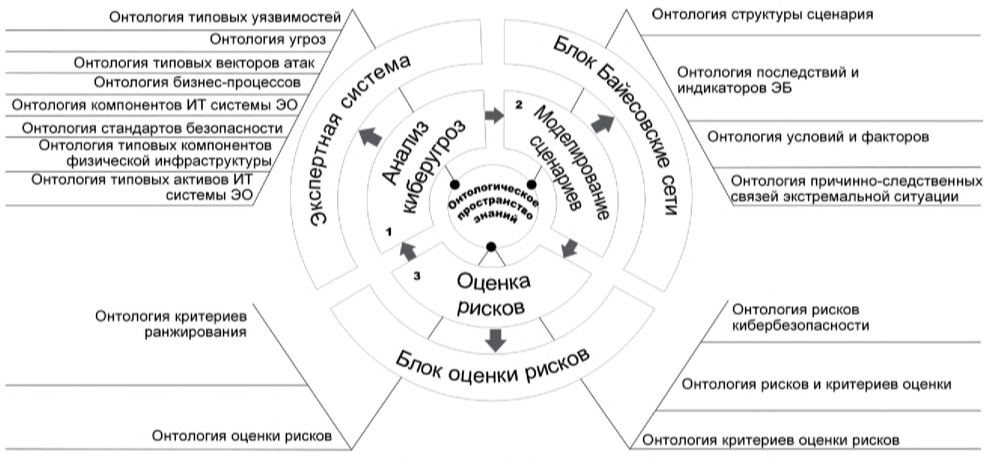
\includegraphics[width=1\linewidth]{scheme}}
    \caption{Строение системы онтологий}
    \label{dio}
\end{figure}

Из данной схемы ясно, что для каждой из основных предметных областей создается набор онтологий, связанных
между собой. В разделе, связанным с анализом киберугроз, онтологический инжениринг позволяет систематизировать
информацию об различных информационно-технологических характеристиках конкретных энергетических объектов
и создать базу знаний их уязвимостей и угроз. В последствии она послужит компонентом для алгоритма проведения
аудита безопасности предприятий и моделировании сценариев возможных экстремальных ситуаций.

За сценарное планирование отвечает байесовская сеть доверия. Сами же сценарии включают в себя следующие данные:
факторы, влияющие на возникновение экстремальных ситуаций, уязвимостей ИТС объекта, природу самой угрозы,
последствия реализации угрозы. В данном случае онтологический инжениринг применяется для создания онтологии
экстремальных сценариев. Конечным результатом работы данной сети должна стать оценка вероятности наступления
того или иного опасного события. При создании множества сценариев их результаты объединяются в онтологию
последствий. В дальнейшем эта онтология служит базой знаний для оценки рисков.

Финальным этапом обработки информации о киберугрозах является оценивание рисков, полученных на основе базы
знаний с вероятностями различных экстремальных ситуаций. Риск рассматривается как комбинация последствий
произошедшего события и возможности его возникновения. Если при анализе рисков обнаружена уязвимость, это
позволяет определить критические факторы возникновения киберугроз на предприятии.

\section{Интеллектуальные системы и кибербезопасность в бизнесс-среде}
Второй, но оттого не менее важной областью применения ИС для обеспечения информационной безопасности
является бизнесс-среда. В данном случае многоагентный подход находит широкое применение в
областях, требующих решения сложных задач: реинжиниринг бизнес-процессов,
построение виртуальных предприятий, имитационное моделирование интегрированных производственных систем
и т.д \cite{mob}. Наибольшую сложность в теоретических исследованиях и практических реализациях современных
многоагентных систем представляют вопросы, связанные с обеспечением информационной безопасности агентов и информационных
ресурсов, которыми они оперируют, в открытых многоагентных виртуальных средах.

В качестве примера автор работы \cite{mob} приводит решение задачи
обеспечения информационной безопасности в объектах многоагентной
системы информационной поддержки инноваций, реализующей
открытую многоагентную виртуальную бизнес-среду инновационной деятельности.

С точки зрения общей логики функционирования такая среда имеет многоагентную реализацию.
Агентная ориентированность выражается в том, что в ней каждый субъект инновационной деятельности
представлен одним или несколькими мобильными агентами, которые представляют предложения
своих владельцев и реализуют процедуры автоматизированного поиска партнеров для сотрудничества.

В общем случае такая многоагентная система, какая описана в работе \cite{mob}, задается отношением множеств
пользователей системы, ее агентов, представляющих их интересы в бизнесс-среде, множества узлов системы,
множества виртуальных бизнесплощадок, множества информационных ресурсов системы, множества атрибутов объектов модели.
Два основных типа агентов системы: мобильные агенты и управляющие агенты. Первые перемещаются между узлами сети,
а вторые координируют процессы взаимодействия и миграции первых.

Для решения задачи обеспечения кибербезопасности в распределенной многоагентной системе авторами статьи \cite{mob}
предлагается метод формирования комплексной самоорганизующейся системы децентрализованного управления безопасностью
мобильных агентов, аутентификация мобильных агентов в которой осуществляется через открытые ключи и
удостоверяющие их центры.

В предлагаемой системе формирование удостоверяющих центров будет осуществляться автоматически на основе механизмов
самоорганизации агентов а функции управления процедурой выдачи сертификатов будут возложены на программных
управляющих агентов.

Самоорганизация заключается в автоматическом формировании виртуальных площадок, объединяющих
агентов с близкими целями в коалиции, и генерации управляющих агентов, выполняющих функции удостоверяющих центров
сертификации, для каждой площадки.

Система безопасности мобильных агентов может быть как централизованной, так и децентрализованной.

В случае использования системы с \textbf{централизованным} управлением безопасностью мобильных агентов в
открытой многоагентной виртуальной бизнес-среде, оно реализуется на выделенном сервере, функциональная
структура которого состоит в следующем: сервер безопасности мобильных агентов обеспечивает
централизованное хранение информации об агентах системы, доступных узлах, виртуальных бизнес-площадках,
открытых ключах агентов, доступ к которым имеют только управляющие агенты системы. Здесь же реализуются
модуль шифрования и дешифрования данных, а также система мониторинга, анализа и моделирования поведения
агентов системы, которая также доступна управляющим агентам системы.

В случае использования системы с \textbf{децентрализованным} подходом управление безопасностью мобильных агентов
в виртуальной бизнес-среде реализуется на каждом из серверных узлов системы
(порталов), на которых пользователи регистрируют свои предложения. При таком решении система безопасности
мобильных агентов является
частью агентного представительства серверного узла и выполняет аналогичные функции, что и сервер безопасности
мобильных агентов: хранит информацию об агентах системы, доступных узлах, виртуальных бизнес-площадках,
открытых ключах агентов, доступ к которым имеют только управляющие агенты системы, реализует процедуры
шифрования и дешифрования данных агентов, осуществляет мониторинг, анализ и моделирование поведения агентов
системы.

Централизованная система в сравнении с децентрализованной обладает рядом недостатков \cite{probs}: % Проверить что цитата по теме
\begin{enumerate}
    \item уязвимость центрального звена (при отказе сервера безопасности
    нарушается защита активных компонентов и всей системы в целом, ее безопасность становится под угрозой);
    \item высокая нагрузка на центральный сервер управления безопасностью при большом количестве агентов
    и узлов и, как следствие – ограниченная масштабируемость;
    \item централизованное администрирование подразумевает полный контроль над ресурсами на стороне сервера,
    что не всегда приемлемо, если ресурсы принадлежат разным пользователям
\end{enumerate}

Помимо описанных выше минусов, согласно работе \cite{mob}, централизованное управление безопасностью
гораздо менее продуктивно и намного более длительно чем децентрализованное. При увеличении количества
узлов и мобильных агентов увеличивается нагрузка на центральный
сервер безопасности мобильных агентов, тем самым уменьшается производительность МАС.

Ввиду описанных выше аспектов, использование децентрализованной системы для обеспечения
безопасности мобильных агентов предпочтительно.
% TODO Дописать этот раздел

\section{Потенциал интеллектуальных систем в информационной безопасности транспорта}
% TODO Дописать этот раздел (одна статья с концептом)
\newpage

\section{Другие идеи для применения интеллектуальных систем в кибербезопасности}
Интеллектуальные системы применяются в контексте кибербезопасности не только в тех областях, о которых было
написано выше. Существуют и не совсем обычные проекты, связанные с этой отраслью.

\subsection{Разработка экспертной системы для контроля информационной безопасности}
Работы \cite{scheme, ontoling} интегрировали в свои интеллектуальные системы экспертную систему ``Cyber''.
Но они не единственные, кто принял решение внедрить экспертную систему в область безопасности информационного
пространства. В работе \cite{idea} автор, ориентируясь на различные банковские и бизнесс структуры, делает акцент на
доступности экспертной системы для пользователя. Поэтому он предлагает собственную архитектуру экспертной системы
(рис. \ref{arch}). Такая архитектура позволяет упростить работу с экспертной системой как со стороны пользователей,
так и со стороны ее проектировщиков.

\begin{figure}[h]
    \center{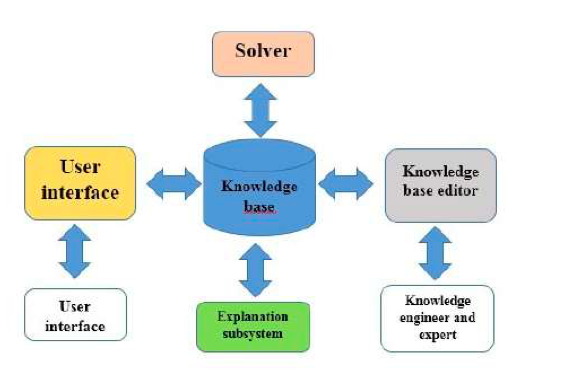
\includegraphics[width=11cm, height=6cm]{arch}}
    \caption{Архитектура экспертной системы \cite{idea}}
    \label{arch}
\end{figure}

Разработка данной экспертной системы состоит из нескольких этапов:
\begin{enumerate}
    \item
    Идентификация
    \item
    Концептуализация
    \item
    Формализация
    \item
    Реализация
    \item
    Тестирование
    \item
    Опытная эксплуатация
\end{enumerate}

На этапе \textbf{идентификации} определяются решаемые задачи, определяются цели разработки,
определяются эксперты и типы пользователей. Во время \textbf{концептуализации} проводится
содержательный анализ проблемной области, выявляются используемые понятия и их взаимосвязи,
определяются методы решения проблемы. После этого при \textbf{формализации}
выбираются и определяются способы представления всех видов знаний, формализуются основные
понятия, определяются способы интерпретации знаний, моделируется работа системы, способы
представления и манипуляции знаниями.

После этого наступает длительная ступень \textbf{реализации}. На этом этапе база знаний
заполняется экспертами и эта часть процесса самая важная и трудоемкая, поскольку происходит
упорядочение знаний, полученных от экспертов, что обеспечивает эффективную работу системы
в дальнейшем и представление знаний в виде ЭС. Реализация выполняется инженером по знаниям.
Стоит помнить, что начиная с этого этапа могут возникнуть определенного рода проблемы \cite{idea}.

Следующим шагом на пути к претворению в жизнь экспертной системы станут различного рода \textbf{тесты}.
На этом этапе выделяются ключевые проблемы проектируемой системы: какую информацию защищать, где она
расположена в базе знаний, какие устройства пользуются базой знаний, достаточно ли надежны пароли,
задаваемые пользователями и т. д... Для их решения задаются необходимые переменные и строятся логические
блоки с ветвлениями. После этого получается готовый продукт, достаточно удобный для потребителей.

\subsection{Применение онтологий в информационных войнах}
Понятие информационной войны подразумевает использование информационных и коммуникационных
технологий для достижения преимуществ по сравнению с потенциальным противником. В данном контексте
информационные структуры рассматриваются как системы, хранящие информацию, обрабатывающие ее и определяющие,
представляет тот или иной пакет угрозу или нет. Для этой цели используется онтологический подход к созданию
интеллектуальной системы, предоставляющей базу знаний для потенциального обучения на ней нейронной сети
или иной самообучающейся системы \cite{wars}. В работе \cite{wars} приводится пример онтологии, с помощью которой
можно определить киберугрозу. Структуру такой онтологии можно увидеть на рис. \ref{ont}.

\begin{figure}[h]
    \center{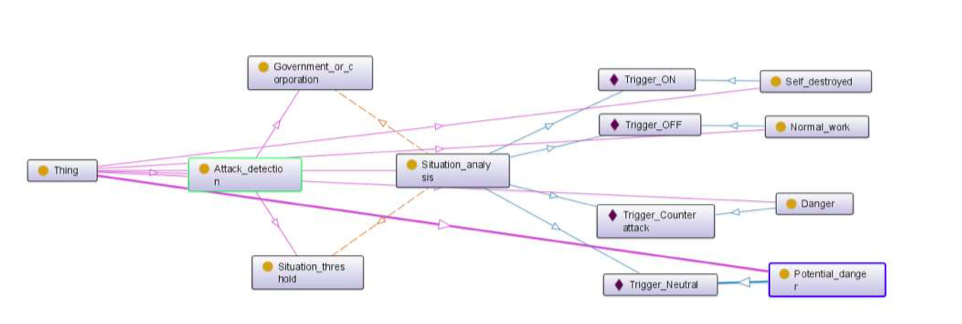
\includegraphics[width=1\linewidth]{ontology}}
    \caption{Структура онтологии для определения угроз \cite{wars}}
    \label{ont}
\end{figure}

Ключевыми звеньями в данной цепочке являются онтологии Attack-detection и Situation threshold.
Первый анализирует на какую информационную систем
% TODO Здесь подробнее написать про то, кто каждая компонента представляет (см статью)


\section{Заключение}
В заключении стоит сказать, что применение интеллектуальных систем в области компьютерной безопасности
достаточно широко. Были рассмотрены как уже созданные модели ИС, так и концепции, которые могут
быть реализованы в будущем. По итогам работы можно сделать вывод, что ИС используются:
%  Написать где используются


Но их работа далеко не всегда бывает быстрой и продуктивной \cite{mob, upg}. Это означает,
что следует и дальше развивать рассмотренные в данной работе технологии использования интеллектуальных
систем для обеспечения безопасности информационного пространства как крупных организаций и компаний, так
и частных лиц.
\newpage

\section{Список литературы}
\medskip

\begin{thebibliography}{}
\bibitem{spheres}
V. Tabakaeva, V. Selifanov, V. An, S. Bularga, and A. Vorozhtsov,
Intelligent information security management systems,  Trans. Sci. Pap. Novosib. State Tech. Univ., vol. 4,
no. 3–4, pp. 165–176., -2020
\bibitem{kognmodels}
Бурый А.С., Усцелемов В.Н. Онтологический подход к формированию когнитивных моделей оценки
кибербезопасности // Информационно-экономические аспекты стандартизации и технического
регулирования.,  No 3. (55). С. 77-84., -2020.
\bibitem{concept}
Зыбин Е.Ю., Кривоноженков В.А., Муллин А.Р., Кохан В.В., Концепция
интеллектуальной системы обеспечения кибербезопасности бортового оборудования
и систем сверхзвукового пассажирского самолета, ФГУП ``ГосНИИАС'', -2021
\bibitem{multigent}
И. В. Котенко, Интеллектуальные механизмы управления кибербезопасностью, -2009.
\bibitem{reqs}
Ворожцова Т. Н., Онтология как основа для разработки интеллектуальной системы обеспечения
кибербезопасности // Онтология проектирования., C.69-77., -2014
\bibitem{scheme}
D. Gaskova, A. Massel, The Technology of Cyber Threat Analysis and Risk Assessment of Cybersecurity
Violation of Critical Infrastructure // Vopr. kiberbezopasnosti, vol. 2, no. 2(30), pp. 42–49, -2019
\bibitem{ontoling}
А. Г. Массель, Д. А. Гаськова, Онтологический инжениринг для разработки интеллектуальной системы анализа угроз
и оценки рисков кибербезопасности энергетических объектов // Онтология проектирования, C. 255-238., -2019
\bibitem{methods}
А. Г. Массель, Методика анализа угроз и оценки риска нарушения информационно-технологической
безопасности энергетических комплексов // XX Байкальской Всероссийской конференции:труды,
т. III., С. 186-195., -2015.
\bibitem{mob}
А.В. Маслобоев, В.А. Путилов, Разработка и реализация механизмов управления информационной безопасностью
мобильных агентов в распределенных мультиагентных информационных системах // Вестник МГТУ, том 13, №4/2,
C. 1015-1032, -2010
\bibitem{probs}
А.В. Маслобоев, М.Г. Шишаев ,  Одноранговая распределенная мультиагентная система
информационноаналитической поддержки инновационной деятельности //
Научно-технический вестник СПбГУ ИТМО, № 4(62), C.108-114, -2009.
\bibitem{idea}
T. Marzhan, Method of development of information security expert system, -2019, [Online].
Available: https://proc.ostis.net/wp-content/uploads/2019/10/OSTIS-2019.pdf
\bibitem{wars}
Научные Труды Конференции, “Open Semantic Technologies for Intelligent Systems”
// Inf.Tsu.Ru, vol. 7740, no. 3, pp. 145-150, -2019,
[Online]. Available: http://www.inf.tsu.ru/library/Publications/2020/2020-139.PDF.
\bibitem{upg}
Коломойцев В.С., Богатырев В.А., Поляков В.И., Open Semantic Technologies for Intelligent Systems
// Inf.Tsu.Ru, vol. 7740, no. 3, pp. 315-320, -2019,
[Online]. Available: http://www.inf.tsu.ru/library/Publications/2020/2020-139.PDF.
\end{thebibliography}

\end{document}
